\documentclass[10pt,a4paper]{article}

% Packages
\usepackage[utf8]{inputenc}
\usepackage{amssymb}
\usepackage{mathtools}
\usepackage{gensymb}
\usepackage{amsmath}
\usepackage{MnSymbol}

\title{\textbf{Mathematical proofs}}
\author{Michal Špano}
\date{March 2022}

\begin{document}

\maketitle

\section{The inner angle of an $n-sided$ convex regular polygon}

% Introduction
Suppose an $n-sided$ convex regular polygon. Its 4 consecutive vertices are shown in the figures, $N_1, N_2, N_3, ..., N_i$ respectively. 
Thus $\Delta_{N_1,N_2,S} \cong \Delta_{N_2,N_3,S}$, i.e. such $n-sided$ polygon consists of $n$ congruent isosceles triangles. 
That is, $|\measuredangle N_2 N_1 S| = |\measuredangle N_1 N_2 S| \implies |\measuredangle N_1 N_2 S| = |\measuredangle S N_2 N_3|$, denoted as $\beta, \beta'$ respectively. 

% Section I
An angle $\alpha = |\measuredangle N_1 S N_2| = \cfrac{360}{n}$, since such an angle multiplied by $n$ makes for a perfect circle of $360\degree$. Likewise $\alpha = 180\degree - 2 \beta$.

% Section I
Let $\Phi$ be an inner angle of the polygon, such that $\phi = 2 \beta$ (shown in the figure at the vertex $N_2$).

% Steps of computations
Express in terms of $\beta$: $\alpha = 180 - 2 \beta \iff \beta = \cfrac{-\alpha + 180}{2}$

Substitute $\alpha$ for $\alpha = \cfrac{360}{n}$: $\beta = \cfrac{-\cfrac{360}{n} + 180}{2} \iff \beta = \cfrac{180n - 360}{2n}$

Express in terms of $\Phi$: $\Phi = 2 \beta = 2 \Big( \cfrac{180n - 360}{2n} \Big) = \cfrac{180n - 360}{n}$ \\

The expression can be further simplified to the following form:

% End of the proof
$$\Phi = \cfrac{(n-2) \pi}{n}$$.

% Include a picture of a unit circle
\begin{figure}[htp]
    \centering
    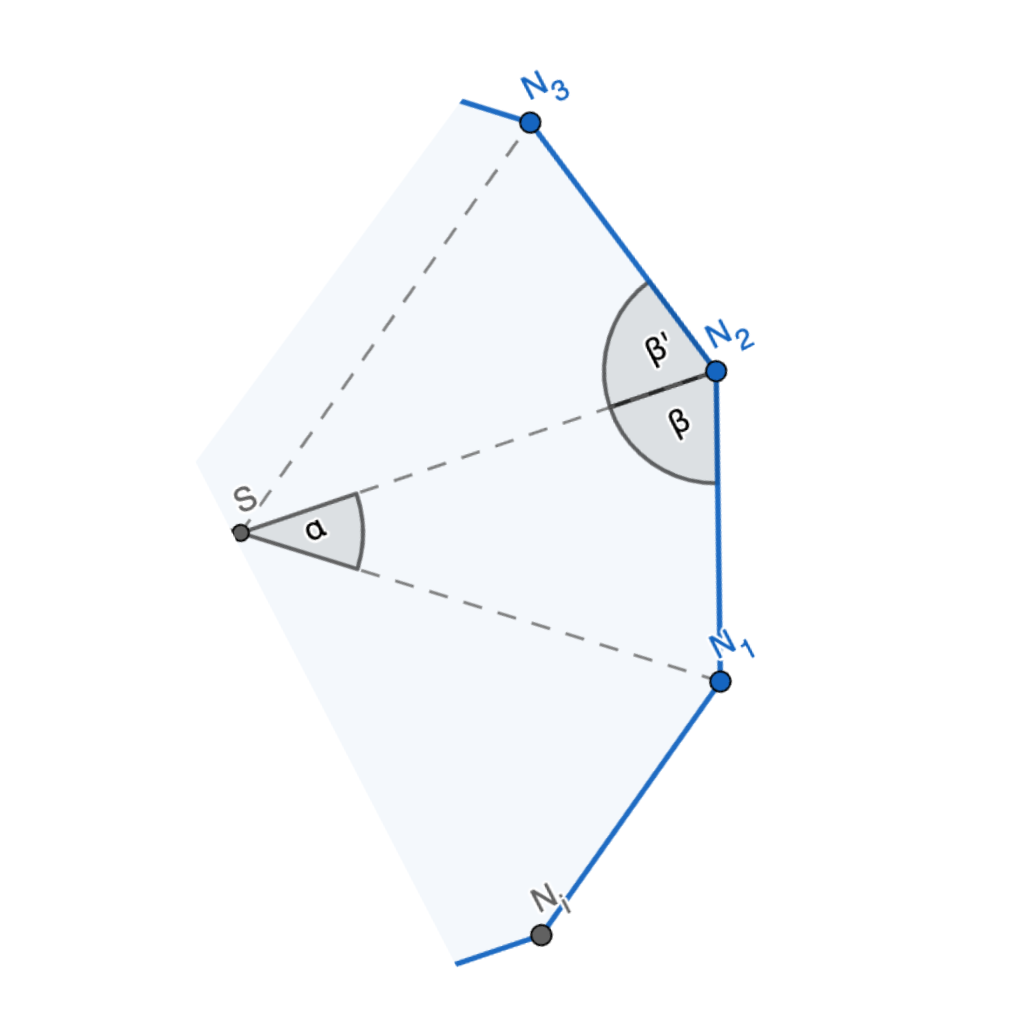
\includegraphics[width=4.cm]{polygon_export.png}
    \caption{$n-sided$ polygon with its 4 vertices in a plane}
\end{figure}

\newpage

\section{The number of diagonals of an $n-sided$ convex regular polygon}

% Steps of the proof
Suppose a geometrical locus of $n$ points on the plane, 
i.e. a set of points $A_1, A_2, ..., A_n$ 
such that $A_1, A_2, ..., A_n$ create an $n-sided$ convex regular polygon.
The number of different abscissas in the geometrical locus is ${n \choose 2}$ 
and denoted as $N_a$. It implies that no abscissa in the locus is given by more than two points, 
i.e. each point is unique. Likewise, $\overlinesegment{A_1A_2} \equiv \overlinesegment{A_2A_1}$ 
holds for any 2 points in the locus, thus such abscissas are counted as one. It can be inferred 
that the number of diagonals, denoted as $N_D$, is the same as \textit{the difference of the number of 
abscissas and the number of sides}: 

% End of the proof
$$N_D = N_s - n$$

\end{document}
